\documentclass[a4paper,12pt]{article} 
\usepackage{mathrsfs}
\usepackage[utf8]{inputenc}
\usepackage[english]{babel}
\usepackage{amsmath}
\usepackage{amsfonts}
\usepackage{amssymb} 
\usepackage{graphicx} 
\usepackage{wrapfig}
\usepackage{enumitem}
\usepackage{fancyhdr}
\usepackage{float}
\usepackage{eurosym}
\usepackage{color}
\usepackage{circuitikz}
\usepackage{titling}
\usepackage{media9}
\usepackage{lipsum}
\usepackage{listings}
\usepackage{tabularx}
\usepackage{tcolorbox}
\usepackage{bookmark}
\usepackage[table]{xcolor}
\definecolor{lightblue}{RGB}{228, 244, 253}
\usepackage{listings}

\definecolor{dkgreen}{rgb}{0,0.6,0}
\definecolor{gray}{rgb}{0.5,0.5,0.5}
\definecolor{mauve}{rgb}{0.58,0,0.82}

\lstset{frame=tb,
  language=Python,
  inputencoding=utf8,
  extendedchars=true,
  aboveskip=3mm,
  belowskip=3mm,
  showstringspaces=false,
  columns=flexible,
  basicstyle={\small\ttfamily},
  numbers=none,
  numberstyle=\tiny\color{gray},
  keywordstyle=\color{blue},
  commentstyle=\color{dkgreen},
  stringstyle=\color{mauve},
  breaklines=true,
  breakatwhitespace=true,
  tabsize=3,
  literate=%
    {á}{{\'a}}1
    {é}{{\'e}}1
    {í}{{\'i}}1
    {ó}{{\'o}}1
    {ú}{{\'u}}1
    {ñ}{{\~n}}1
    {č}{{\v{c}}}1
}
\usepackage[left=3cm,right=3cm,top=3cm,bottom=4cm]{geometry}
\sloppy

\pagestyle{fancy}
\providecommand{\abs}[1]{\lvert#1\rvert}
\providecommand{\norm}[1]{\lVert#1\rVert}

%%% Para las cabeceras
\newcommand{\hsp}{\hspace{20pt}}
\newcommand{\HRule}{\rule{\linewidth}{0.5mm}}
\headheight=50pt
%%% 
\newcommand{\vacio}{\textcolor{white}{ .}}

%%% Para que las ecuaciones se numeren
%%% con el número de sección y el de ecuación.
\renewcommand{\theequation}{\thesection.\arabic{equation}}


% Color azul para algunos 
% textos de la portada
\definecolor{azulportada}{rgb}{0.16, 0.32, 0.75}

%%%% Azul para textos de headings
\definecolor{azulinterior}{rgb}{0.0, 0.2, 0.6}

%%%%%%%%%%%%%%%%%%%%%%%%%%%%%%%%
%%%%%% Datos del proyecto %%%%%%
%%%%%%%%%%%%%%%%%%%%%%%%%%%%%%%%
%%%TÍTULO
%%% Escribirlo en minúsculas, el programa
%%% lo pondrá en mayúsculas en la portada.

\title{laboratory notebook}

%%%% AUTORES
\author{Mathilde Gallego \and Pablo Tuñón \and Jorge Vančo}

%%%%%%%%%%%%%%%%%%%%%
%%%%%%%%%%%%%%%%%%%%
\begin{document}

%%%%%%%%%%%%%%%%%%%%%%%%%%%%%%%
%%%%%%%%%%%%%%%%%%%%%%%%%%%%%%%
\begin{titlepage} %%%%% Aquí no hay que tocar nada.
	%%%% Las siguientes instrucciones generarán automáticamente
	%%%% la portada de tu proyecto.
	%%% Cambio de la estructura de esta página
\newgeometry{left=0.6cm,top=1.3cm,bottom=1.2cm}

\fbox{\parbox[c]{18.5cm}{
\begin{center}
\vspace{1.5cm}
{\fontfamily{ptm}\fontsize{24}{28.8}\selectfont{Universidad Pontificia Comillas}}\\
[3.5em]
{\fontfamily{ptm}\fontsize{24}{5}\selectfont{ICAI}}\\
[4.5em]
\\
[2cm]
{\fontfamily{ptm}\fontsize{24}{5}\selectfont{Dynamic systems}}\\
[2cm]

% Autor del trabajo de investigación
\textcolor{azulportada}{\fontfamily{ptm}\fontsize{16}{5}\selectfont{\theauthor}}\\
[2cm]
% Título del trabajo
\textcolor{azulportada}
{\fontfamily{ptm}\fontsize{30}{5}\selectfont{\textsc{\thetitle}}}\\
%{\Huge\textbf{\thetitle}}\\
[1.2cm]

\includegraphics[width=10cm]{Logo ICAI.png}
\\[1.8cm]

{\fontfamily{ptm}\fontsize{16}{5}\selectfont{Scholar year 2024-2025}}\\
[4cm]
\end{center}
}}

\restoregeometry
\end{titlepage}

\date{} % Eliminar la fecha

\newpage

\renewcommand{\contentsname}{Index}
\tableofcontents
\thispagestyle{empty}


\newpage


\section{Lab 1: Forced response}


\vspace{1cm}

\subsection{Pre-laboratory work}

\vspace{0.5cm}

The requirements to complete the pre-laboratory work were the following: watching a video that explains some functions to work in Matlab with forced responses, stating two differential equations in their Laplace transform of the following circuit:

\vspace{0.5cm}

\begin{figure}[H]
    \centering
    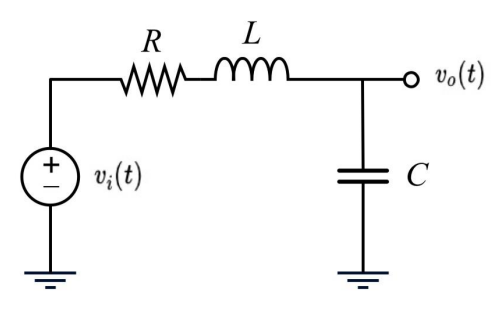
\includegraphics[width=0.5\linewidth]{circuit_lab_1.png}
    \caption{Circuit to analyze, pre-laboratory work 1}
    \label{fig:Lab 1 circuit}
\end{figure}

\vspace{0.5cm}

\begin{equation}
\frac{V_0(s)}{V_i(s)} = \frac{1}{CLs^2 + CRs + 1} 
\end{equation}
\begin{equation}    
\frac{I(s)}{V_i(s)} = \frac{Cs}{CLs^2 + CRs + 1}
\end{equation}

\vspace{0.5cm}

On top of obtaining the Laplace transform of the differential equations, it was as well required to provide a value for R that produces two equal real poles. To achieve that the roots of the polynomial of the denominator of (1.1) had to be equal, which means that the discriminant \(\bigtriangledown=b^2-4ac\) has to be equal to 0:

\vspace{0.5cm}

\[
\bigtriangledown = 0 \implies (CR)^2 - 4CL = 0 \iff R = 2\sqrt{\frac{L}{C}}
\]

\vspace{0.5cm}

\subsection{Laplace transform of the equations}

\vspace{0.5cm}

To obtain the Laplace transform to (1.1) and (1.2) a function \textit{RLC} was created that received values for the R, L and C of the circuit as well as the mode of transform that should be applied and returns the transform of (1.1) and (1.2) using: \textit{tf}, \textit{zpk} or symbolic \textit{s}. The three models create the same function, this can be observed on the following Bode diagrams where only one of the 3 functions is visible as the functions overlap:

\vspace{0.5cm}

\begin{figure}[H]
    \centering
    \begin{minipage}[b]{0.40\linewidth}
        \centering
        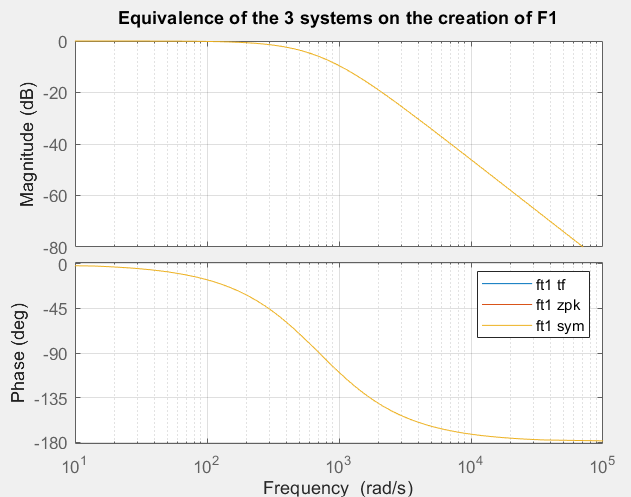
\includegraphics[width=\linewidth]{equivalence f1.png}
        \caption{Transfer function of (1.1) with different methods, own authorship.}
        \label{fig:equivalence-f1}
    \end{minipage}
    \hspace{0.05\linewidth} % Espacio entre las dos imágenes
    \begin{minipage}[b]{0.40\linewidth}
        \centering
        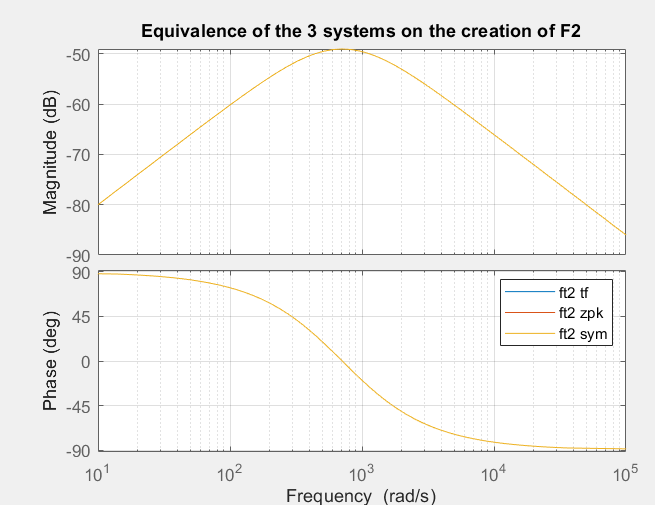
\includegraphics[width=\linewidth]{equivalence f2.png}
        \caption{Transfer function of (1.2) with different methods, own authorship.}
        \label{fig:equivalence-f2}
    \end{minipage}
\end{figure}

\vspace{0.5cm}

The equivalence can also be seen as the \textit{zpkdata} and the \textit{dcgain} are shared between the three implementations:

\vspace{0.5cm}

{\centering
$z_1$ = [ ] \\ 
$p_1$ = [$-7.0711e+02, -7.0711e+02$] \\
$k_1$ = $1/CL$\\
DC Gain 1= $1$\\
$z_2$ = $0$ \\
$p_2$ = [$-7.0711e+02, -7.0711e+02$] \\
$k_2$ = $1/L$\\
DC Gain 2 = $0$
}
\newpage

\subsection{Inverse Laplace transform of the equations}

\vspace{0.5cm}

Given that the three functions are equivalent, their residues (which are the numerators of the simple fractions decomposition of the transference function) are equal. 

The residues can be obtained by using the function \textit{residues} applied to the transfer function, regardless of the construction method. \\

{\centering
$r_1$=$5$ \\
$r_2$= $-3535.53390593274$\\
}

\vspace{0.5cm}
%however, given the high amount of residues and the finite document, those are only contained on the associated Matlab document \textit{Lab1.m}. 
When applying a step function of value 2 to the functions )(1.1) and (1.2) with the method \textit{step} a set of values are returned. By plotting the values it can be seen the inverse Laplace transform (on the time domain) of the transfer function after applying a step function:

\vspace{0.5cm}

\begin{figure}[H]
    \centering
    \begin{minipage}[b]{0.40\linewidth}
        \centering
        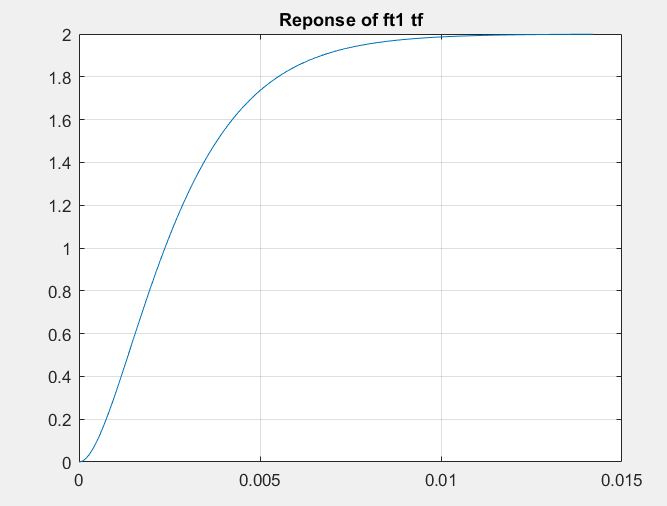
\includegraphics[width=\linewidth]{tf1 response.png}
        \caption{Response of (1.1) calculated with \textit{tf} to a step 2 function, own authorship.}
        \label{fig:tf1-response}
    \end{minipage}
    \hspace{0.05\linewidth} % Espacio entre las dos imágenes
    \begin{minipage}[b]{0.40\linewidth}
        \centering
        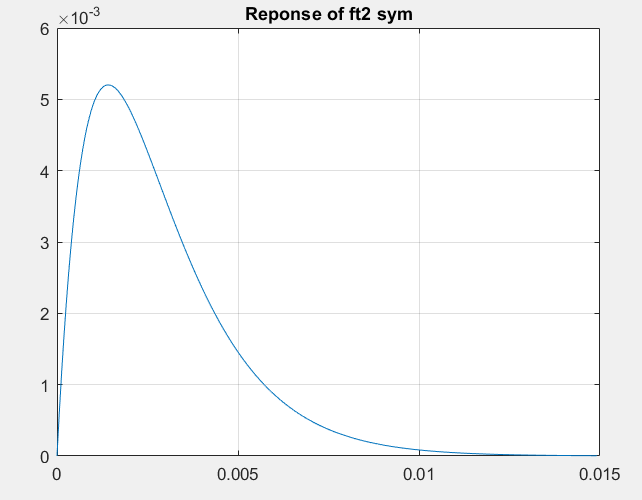
\includegraphics[width=\linewidth]{sym2 response.png}
        \caption{Response of (1.2) calculated with \textit{sym} to a step 2 function, own authorship.}
        \label{fig:sym2-response}
    \end{minipage}
\end{figure}

\vspace{0.5cm}

\subsection{R variations}

\vspace{0.5cm}

All the previous work has been done with an R that allows double real poles, however, through this subsection it will be studied the effects on the previous work of a variation of the value of the resistance of the Figure 1. the values for R that will be taken into consideration are 3:

\vspace{0.5cm}

\[ R_1 = 100\ \Omega\]
\[R_2 = 2 \sqrt{\frac{L}{C}} \simeq 282.84\ \Omega\]
\[R_3 = 500\ \Omega\]

\vspace{0.5cm}

To simplify and reduce the number of equations and figures to take into account, the study will only be performed on (1.1) built with the method \textit{tf} as the analysis of the other 2 modes and transfer function is equivalent. The first observation (other than a variation on the values of the transfer function) that can be made are the poles of the transfer function:

\vspace{0.5cm}

\[\text{Poles \ of} \ (1.1) \text{associated to} \ R_1 = -250 \pm 661.44i\]
\[Poles \ of \ (1.1) \ associated \ to \ R_2 = -707.11\ \text{(double pole)}\]
\[Poles \ of \ (1.1) \ associated \ to \ R_3 =   -2280.8; 219.22\]

\vspace{0.5cm}

Given the poles, it is expected that the complex conjugated poles would provide a response function that would oscillate before achieving stability. Between the poles of \(R_2\) and \(R_3\), the response that corresponds to \(500\Omega\) should achieve stability faster as it has the higher pole in absolute value. However, as it also has a positive pole, that makes the speed at which it converges to the stable value lower than the one with 2 real poles, this can be seen on the following figure:

\vspace{0.5cm}

\begin{figure}[H]
    \centering
    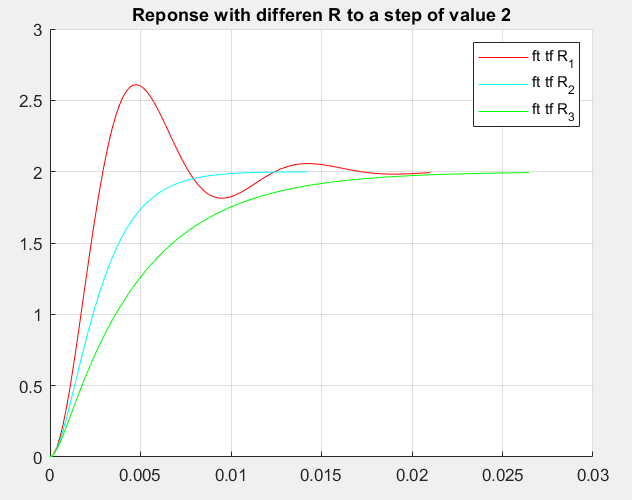
\includegraphics[width=0.5\linewidth]{response diff r.png}
    \caption{Responses of Rs when applied to (1.1) calculated with \textit{tf}, own authorship}
    \label{fig:response-diff-r}
\end{figure}

\vspace{0.5cm}

The previous analysis was produced for the forced response, however, the circuit is not fully modeled and solved until the free response is taken into account. As there are some initial conditions \(i(0^-) = 5mA \ V_0(0^-) = 2V\) the free response can be calculated through the following equation where R can be substituted depending on the value of the resistor of the circuit:

\vspace{0.5cm}

\begin{equation}
    Y_l = \frac{CLV_0(0^-)s + LI(0^-) + CRV_0(0^-)}{CLs^2 + CRs + 1}
\end{equation}

\vspace{0.5cm}

\subsection{Applications}

\vspace{0.5cm}

Through the entire laboratory there where provided functions and methods to calculate the different responses \(y_f, y_l\) as well as the Laplace transform and the inverse Laplace transform, therefore all the tools to solve a real problem were provided. The exercise 2.7 will be solved to proof the correct work of the functions. Firstly the Laplace transform of the circuits ODE:

\vspace{0.5cm}

\begin{equation}
    y_f = \frac{1/R}{s^2 + (1/(5R) + 5R)s + 2} . \frac{5}{s}
\end{equation}

\begin{equation}
    y_l = \frac{s/R + (1/R)(1/(5R) + 5R)}{s^2 + (1/(5R) + 5R)s + 2}
\end{equation}

\vspace{0.5cm}

After stating the transfer function and the free response (both in the Laplace space), it is needed to calculate the two values of R that create two exponentials with 1ms and 5ms (\(\tau_1 \ and \tau_2\)):

\vspace{0.5cm}

\[ Expected \ response(t) \ = Ae^{-ats}\gamma(t) + Be^{-bts} \]
\[\tau_1 = \frac{1}{-a} \implies a = -1 \ ; \tau_2 = \frac{1}{-b} \implies b = -2\]
\[Expected \ response(s) = \frac{A}{s-a} + \frac{B}{s-b}\]

\vspace{0.5cm}

The previous results imply that the roots of the denominator of (1.4) should be a and b, hence obtaining:

\vspace{0.5cm}

\[R = 76.4\Omega \ or \ R = 524\Omega\]

\newpage

Taking the biggest R from the pair, the total response can be calculated. However it is worth to highlight the following: to obtain the function on the time \textit{step(5)} was used for the \(Y_f\) and \textit{impulse} for \(Y_l\) . The result of the calculus of the problem is expressed in the following figure:

\vspace{0.5cm}

\begin{figure}[H]
    \centering
    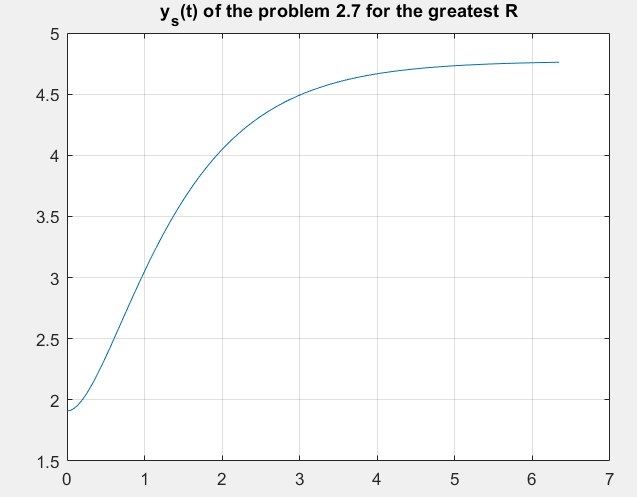
\includegraphics[width=0.35\linewidth]{solution.png}
    \caption{Response solution to the exercise 2.7 for the greatest R, own authorship}
    \label{fig:2-7-sol-response}
\end{figure}

\newpage


\section{Lab 2: Transient response}


\vspace{1cm}

\subsection{Pre laboratory work}
\vspace{0.5cm}

To prepare the second laboratory, it was required to watch a video detailing the use of Simulink besides other functions of use. It was also needed to study the circuit showed below, or more precisely to compute, $v_o(t)$ and $i(t)$ in Laplace's domain as a function of other variables of the circuit (R,L and C).

\vspace{0.5cm}

\begin{figure}[H]
    \centering
    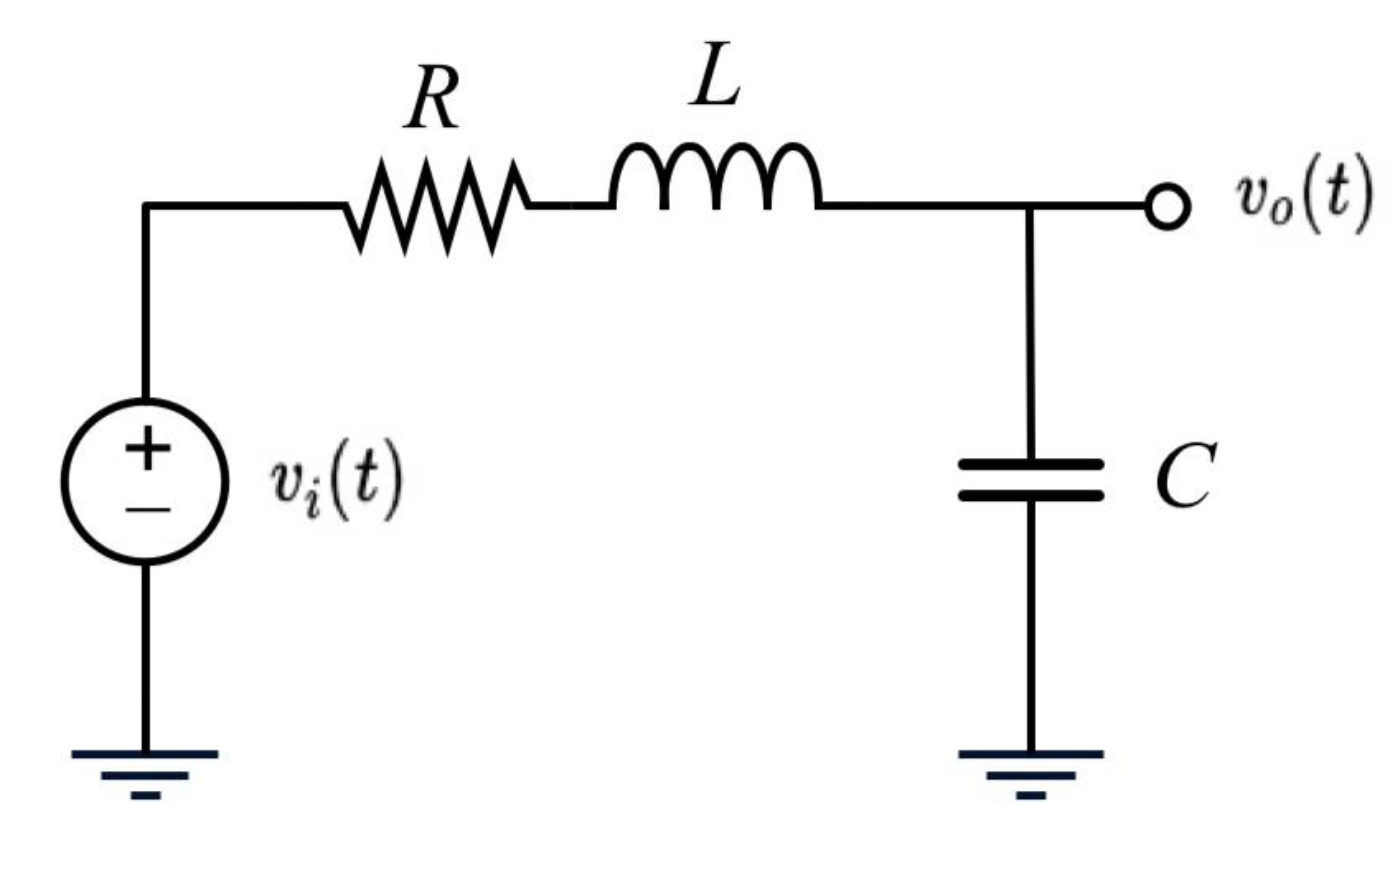
\includegraphics[width=0.5\linewidth]{circuit_lab_2.png}
    \caption{Circuit to analyze, pre-laboratory work 2}
    \label{fig:enter-label}
\end{figure}

\vspace{0.5cm}

As the intensity is the same in the loop, a voltage divider can be used to get $V_o(s)$ which is equal to the difference in potential before and after C. Thus obtaining :

\[V_o(s)= \frac{1/Cs}{R+Ls+1/Cs}Vi(s)= \frac{1}{LCs^2+RCs+1 }Vi(s)\]

Then, 

\begin{equation} 
\frac{V_o(s)}{V_i(s)}=\frac{1}{LCs^2+RCs+1 }
\end{equation}

\vspace{0.5cm}

To obtain $I(s)$, it can be used: $i(t)=C\frac{dv_c}{dt}$. Knowing $v_c(t)=v_o(t)$ so in the Laplace Domain: $I(s)=C \cdot sV_o(s)$ : 

\vspace{0.5cm}

\begin{equation}
\frac{I(s)}{V_i(s)}=\frac{Cs}{LCs^2+RCs+1 }
\end{equation}

\vspace{1cm}

% To compute the free response, it is required to find the initial conditions of the system. For $v_i(t)$ it is needed one initial condition as it is a first order system while $v_o(t)$ provides a second order system with two initial conditions. It is known:

% \vspace{0.5cm}

% \[i(0^-)=I_o;\ v_c(0^-)=V_{co}; \ v_i(0^-)=0\]

% \vspace{0.5cm}

% To calculate the transient response, it is also required the derivative of $v_o(t)$ at $t=0^-$, in order to get it, the tensions of the loop are added :

% \vspace{0.5cm}

% \[v_i(t)=R\cdot i + v_L(t) + v_o(t)\]

% \vspace{0.5cm}

% Isolating $v_L(t)$ :

% \vspace{0.5cm}

% \[v_L(t) = L \cdot \frac{di}{dt} = v_i(t)-R\cdot i - v_o(t)\]
% \[\frac{di}{dt} = \frac{1}{L} \left( v_i(t)-R\cdot i - v_o(t) \right)\]

% \vspace{0.5cm}

% Evaluating the expression at $t=0^-$: 

% \vspace{0.5cm}

% \[\frac{di(0^-)}{dt} = \frac{1}{L} \left( 0-R\cdot I_o - V_{co} \right) = \frac{1}{L} \left( R\cdot I_o - V_{co} \right)\]

% \vspace{0.5cm}

The free responses of $V_0(s)$ and $I(s)$ are:

\vspace{0.5cm}

\begin{equation}
    Y_{L_v} = \frac{V_0LCs + LI_0 + V_0RC}{CLs^2 + CRs + 1}
\end{equation}

\vspace{0.5cm}

\begin{equation}
    Y_{L_i} = Yl_vCs - V_0C
\end{equation}

\vspace{0.5cm}

\subsection{Block diagram analysis}

\vspace{0.5cm}

A block diagram is a structure that helps in the resolution of physical systems, the basis of it stands on the equations of the system. These equations include the parameters of the system, variables and a set of integers $1/s$ to represent the differential signs.\\ In the case of the Figure 8, the parameters are the initial conditions of the electrical components as well as their constant values, the variables are the two outputs and the integers are produced by the coil and the capacitor:

\vspace{0.5cm}

\begin{figure}[H]
    \centering
    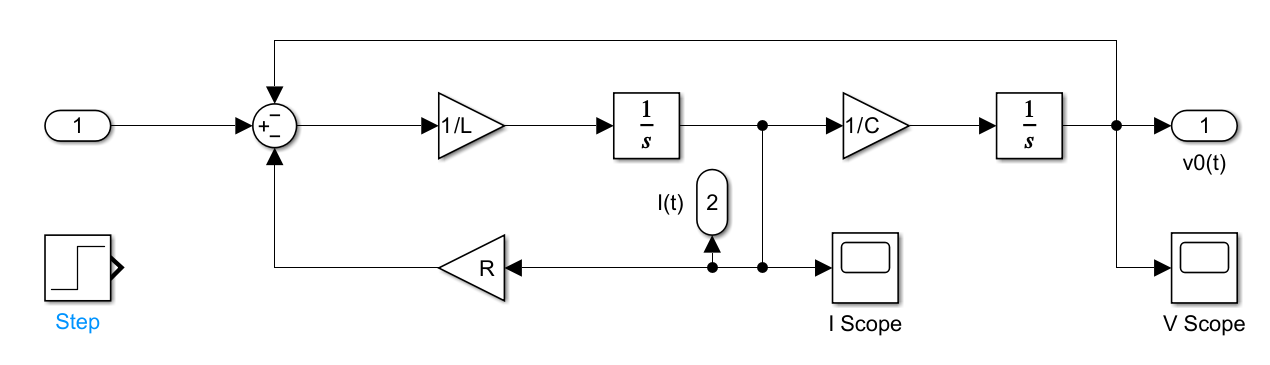
\includegraphics[width=0.75\linewidth]{block diagram.png}
    \caption{Circuit block diagram, own authory}
    \label{fig:Lab 2 circuit}
\end{figure}

\vspace{0.5cm}

Besides of the block diagram that shows $v_0(t)$ as an output with no input, some blocks were added to allow a further analysis:

\begin{enumerate}
    \item Second output: marked as I(t), it is useful as not one but two variables are studied on this system: $v_0(t)$ and $I(t)$.

    \item Scopes I and V: the scope is a block that shows the output function of the circuit, it also allows the user to send the output function to a Matlab script for other than visual analysis.

    \item Step: the block is capable of generating a step function of a given value, on this context it is used to vary the input of the system, aiming for a richer comprehension.
\end{enumerate}

It is worth mentioning that the initial values and parameters are controlled through the associated \textit{Lab2.m} file. The outputs of the system at the corresponding scopes are the following:

\vspace{0.5cm}

\begin{figure}[H]
    \centering
    \begin{minipage}[b]{0.4\linewidth}
        \centering
        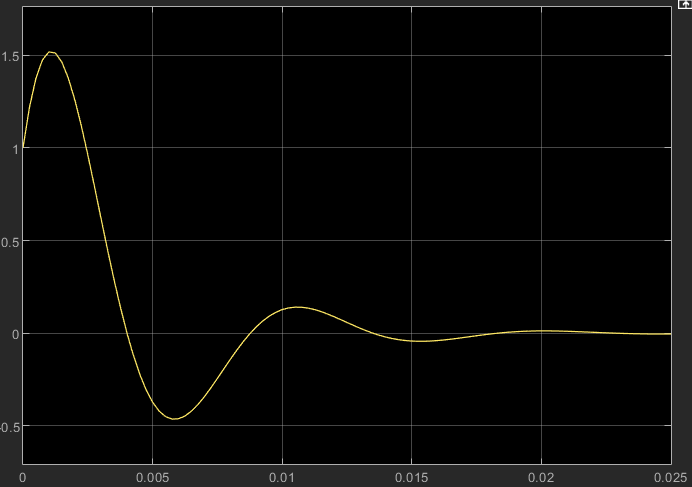
\includegraphics[width=\linewidth]{scopev.png}
        \caption{Transient response of the $v_0(t)$ scope associated to (2.8), own authorship.}
        \label{fig:scopev}
    \end{minipage}
    \hspace{0.05\linewidth} % Espacio entre las dos imágenes
    \begin{minipage}[b]{0.4\linewidth}
        \centering
        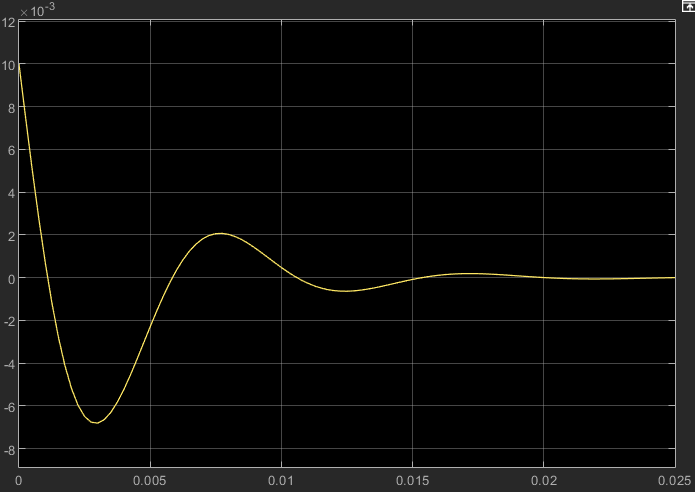
\includegraphics[width=\linewidth]{scopei.png}
        \caption{Transient response of the $I(t)$ scope associated to (2.9), own authorship.}
        \label{fig:scopei}
    \end{minipage}
\end{figure}


\subsection{Responses analysis}

\vspace{0.5cm}

As it was showed on the previous section, the transient response can be obtained not only through analytic methods but also through experimental. Aiming for a fast verification of the similarity of the responses, they will be plotted on a figure. As \textit{impulse} (the function applied to (2.8) and (2.9) to transfer those to the time space) produces 101 values from 0 to 0.025, the sampling time of the scope was modified to be always $0.025/(101-1)$ obtaining 101 points and allowing a correct representation:

\vspace{0.5cm}

\begin{figure}[H]
    \centering
    \begin{minipage}[b]{0.4\linewidth}
        \centering
        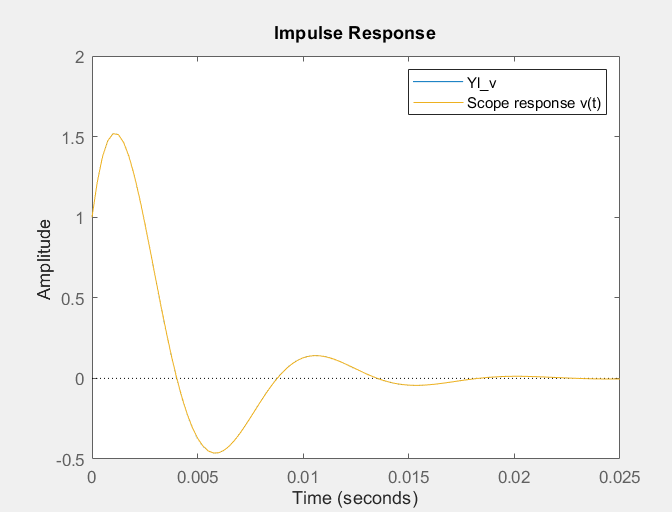
\includegraphics[width=\linewidth]{scopeanalyticalv.png}
        \caption{Transient response of the $v_0(t)$ scope compared with the analytical response (2.8), own authorship.}
        \label{fig:scopeanalyticalv}
    \end{minipage}
    \hspace{0.05\linewidth} % Espacio entre las dos imágenes
    \begin{minipage}[b]{0.4\linewidth}
        \centering
        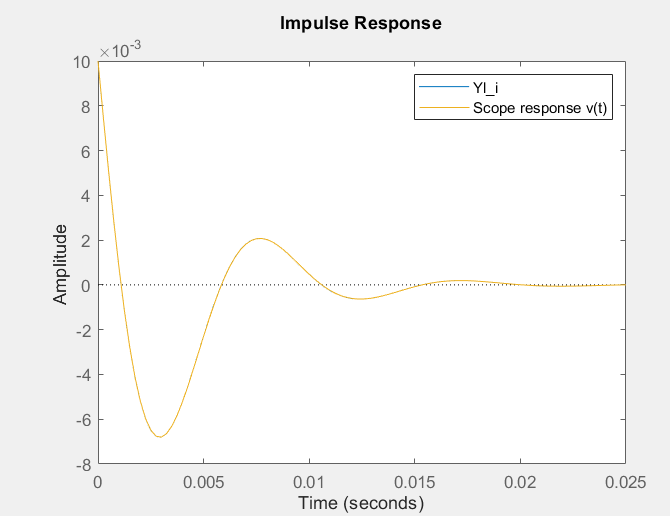
\includegraphics[width=\linewidth]{scopeanalyticali.png}
        \caption{Transient response of the $I(t)$ scope compared with the analytical response (2.9), own authorship.}
        \label{fig:scopeanalyticali}
    \end{minipage}
\end{figure}

It can  be appreciated how the analytical and experimental responses are coincidental, however for a more exhaustive verification, the zpk parameters of the free response where calculated. $v_0(t)$ parameters:

\vspace{0.5cm}

\[z = -1500;\ p = -250 + 661.44i (conjugated); \ k = 1\]

\vspace{0.5cm}

$I(t)$ parameters:

\[z = 500;\ p = -250 + 661.44i (conjugated); \ k = 0.01\]

\vspace{0,5cm}

The previous results are identical for the two methods of calculating the transient response, therefore it has been proved that the methods are equivalent. 

\vspace{0.5cm}

It is worth to mention that the transfer response can also be obtained through the block diagram. The function \textit{linmod} can be applied to a simulink block diagram file, to obtain the numerators and denominators of the different transfer functions of the diagram. To verify the correction of the function, the functions were generated to compare with the zpk and the gain values of the analytical resolutions obtaining a perfect match:

\vspace{0.5cm}

{\centering
$z_v$ = [ ] \\ 
$p_v$ = [$-250 + 661.44i (conjugated)$] \\
$k_v$ = $1/CL$\\
$DC\ Gain_v$ = $1$\\
$z_i$ = $0$ \\
$p_i$ = [$-250 + 661.44i (conjugated)$] \\
$k_i$ = $1/L$\\
$DC\ Gain_i$ = $0$\\
}

\vspace{0.5cm}

\subsection{Parameter modifications}

\vspace{0.5cm}

The parameters can be modified as in the first laboratory to show different type of systems, if the R takes the value of $500\Omega$, the system is still a over-damped system, however it is less damped (this result is only studied with the $Yl_v$ as they share denominator). It is also important to note that although the over-damp factor is only defined for second order systems without zeros, it will be used also in this system with an equal objective instead of a poles magnitude analysis:

\vspace{0.5cm}

\[For \ R \ = \ 100\Omega \implies Yl_v(s) =\frac{2\cdot10^{-6}s + 0.003}{2\cdot10^{-6}s^2 + 0.001s + 1} \implies \zeta = \frac{0.001\cdot5\cdot10^5}{2\sqrt{5\cdot10^5}} \approx 0.01\]

\[For \ R \ = \ 500\Omega \implies Yl_v(s) = \frac{2\cdot10^{-6}s + 0.007}{2\cdot10^{-6}s^2 + 0.005s + 1} \implies \zeta = Yl_v(s) = \frac{0.005\cdot5\cdot10^5}{2\sqrt{5\cdot10^5}} \approx 0.05\]

\vspace{0.5cm}

This greater damping factor can also be appreciated on the graphs of the responses, the oscillations are almost nonexistent:

\vspace{0.5cm}

\begin{figure}[H]
    \centering
    \begin{minipage}[b]{0.45\linewidth}
        \centering
        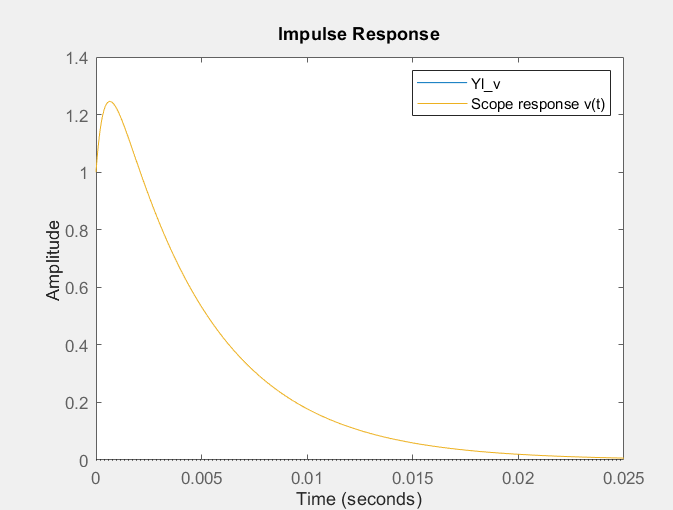
\includegraphics[width=\linewidth]{scopeanalyticalmodifiedv.png}
        \caption{Transient response of the $v_0(t)$ scope compared with the analytical response (2.8) and a modified R, own authorship.}
        \label{fig:scopeanalyticalmodifiedv}
    \end{minipage}
    \hspace{0.05\linewidth} % Espacio entre las dos imágenes
    \begin{minipage}[b]{0.45\linewidth}
        \centering
        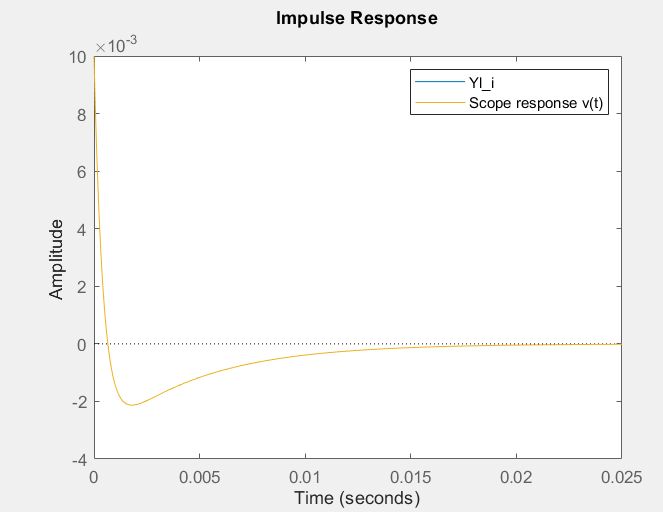
\includegraphics[width=\linewidth]{scopeanalyticalmodifiedi.png}
        \caption{Transient response of the $I(t)$ scope compared with the analytical response (2.9) and a modified R, own authorship.}
        \label{fig:scopeanalyticalmodifiedi}
    \end{minipage}
\end{figure}

\vspace{0.5cm}

Furthermore, as it was exposed in some previous sections, the input of the circuit can be changed from a null signal to a step function, therefore, the outputs on the scopes will show the transient response added to the forced response. The step function has been taken with a value of 2 and $R = \Omega$:

\vspace{0.5cm}

\begin{figure}[H]
    \centering
    \begin{minipage}[b]{0.45\linewidth}
        \centering
        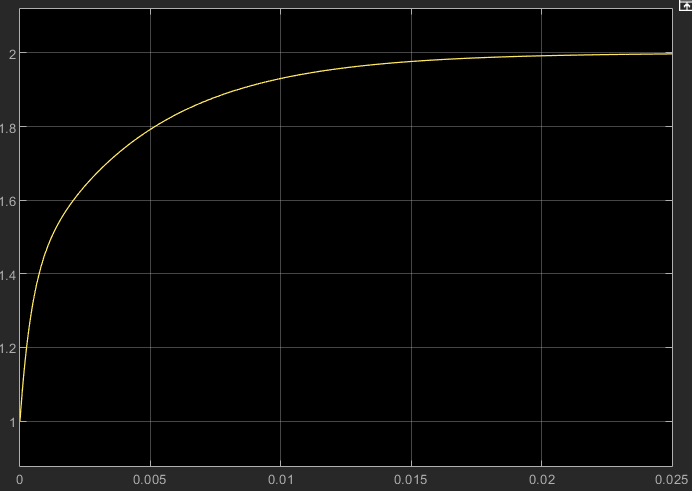
\includegraphics[width=\linewidth]{scopevstep.png}
        \caption{Total response of $v_0(t)$ to a step function with a modified R, own authorship.}
        \label{fig:scopevstep}
    \end{minipage}
    \hspace{0.05\linewidth} % Espacio entre las dos imágenes
    \begin{minipage}[b]{0.45\linewidth}
        \centering
        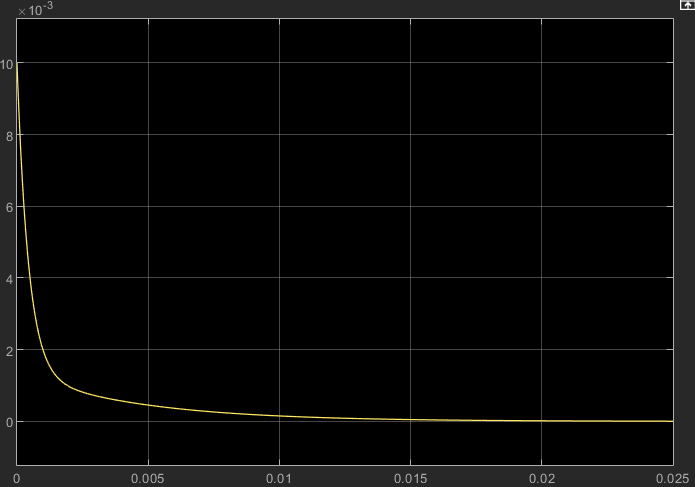
\includegraphics[width=\linewidth]{scopeistep.png}
        \caption{Total response of $I(t)$ to a step function with a modified R, own authorship.}
        \label{fig:scopeistep}
    \end{minipage}
\end{figure}

\vspace{0.5cm}

To fully show the equality of the analytical and experimental methods to calculate different responses of the system, by making 0 all the initial conditions and applying a step function to the system, the forced responses can be obtained. The $v_0(t)$ is identical to the green function of the figure 6 of the notebook. Additionally, the $I(t)$ follows the physical rules of the capacitors, before the steady state $I(t) = I_c(t)$ however, as time passes, the capacitor works as an open circuit, which implies that no intensity will be found on the capacitor and that $I(t) \neq I_c(t)$

\vspace{0.5cm}

\begin{figure}[H]
    \centering
    \begin{minipage}[b]{0.45\linewidth}
        \centering
        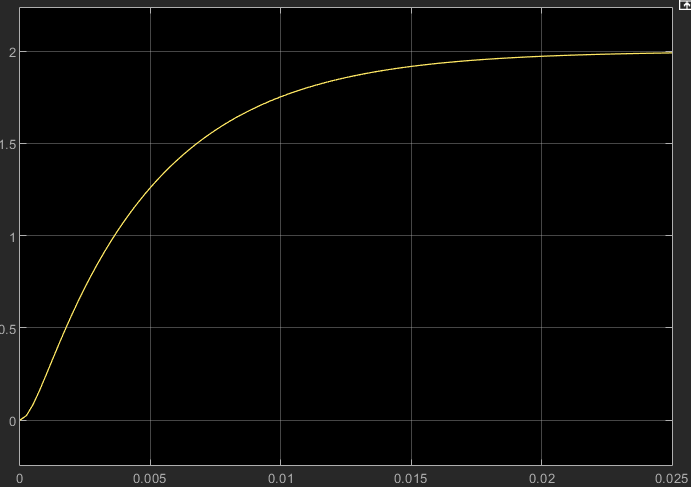
\includegraphics[width=\linewidth]{scopevstep0.png}
        \caption{Forced response of $v_0(t)$ to a step function with a modified R, own authorship.}
        \label{fig:scopevstep0}
    \end{minipage}
    \hspace{0.05\linewidth} % Espacio entre las dos imágenes
    \begin{minipage}[b]{0.45\linewidth}
        \centering
        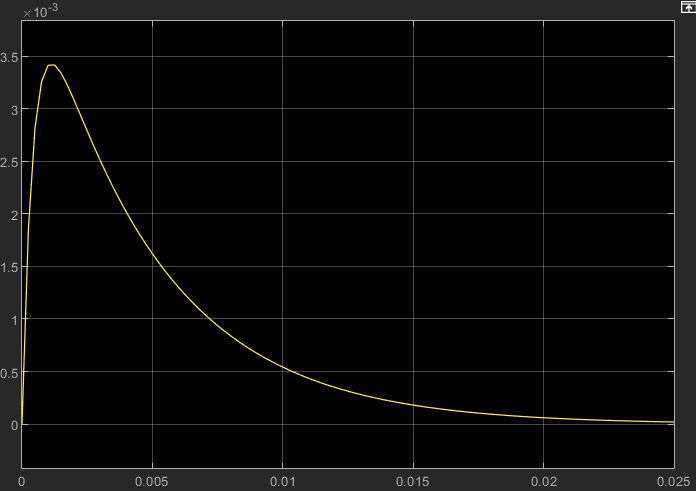
\includegraphics[width=\linewidth]{scopeistep0.png}
        \caption{Forced response of $I(t)$ to a step function with a modified R, own authorship.}
        \label{fig:scopeistep0}
    \end{minipage}
\end{figure}

\vspace{0.5cm}

\end{document}  
